\documentclass[xcolor=table]{beamer}

\usepackage{graphicx}
\usepackage{wrapfig}
\usepackage{url}

\title{GV120 - Politics and Economics Policies}
\subtitle{University of Essex - Department of Government}
\date{Week 3 -- 18 October, 2019}				% or you can specify a date, just write it down instead of "\today"
\author{Lorenzo Crippa} 

\usetheme[progressbar=frametitle]{metropolis}
\usecolortheme{seahorse}						% try others: wolverine; crane...

\begin{document}
\frame{
\titlepage
}

\frame{
\frametitle{Organisation of presentations}
\begin{itemize}
\item Everyone signed up for a presentation?
\item Everyone found their readings on Moodle?
\item Questions or problems?
\end{itemize}

}

\frame{
\frametitle{Seminar timetable}

\begin{table}[]
\centering
\resizebox{8.5cm}{!}{%
\begin{tabular}{|c|l|}
\hline
{\color[HTML]{333333} \textbf{Week number}} & \multicolumn{1}{c|}{{\color[HTML]{333333} \textbf{Groups and activities}}}                                        \\ \hline
{\color[HTML]{333333} 2}                    & {\color[HTML]{333333} Organisation and introduction}                                                              \\ \hline
{\color[HTML]{333333} 3}                    & {\color[HTML]{333333} Henri Maes and Mark Valentini}                                                                           \\ \hline
{\color[HTML]{333333} 4}                    & {\color[HTML]{333333} \begin{tabular}[c]{@{}l@{}}Ester Cavaioni and Blake Mallon\\ Sally Touray\end{tabular}}                                                                           \\ \hline
{\color[HTML]{333333} 5}                    & {\color[HTML]{333333} \begin{tabular}[c]{@{}l@{}}Emma Paulinyova and Emma Sornlund\\ Sònia Villalba\end{tabular}}                                                                           \\ \hline
{\color[HTML]{333333} 6}                    & {\color[HTML]{333333} \begin{tabular}[c]{@{}l@{}}Discuss take-home assignment\\Samuel Leonard and Joshua Kelly\end{tabular}} \\ \hline
{\color[HTML]{333333} 7}                    & {\color[HTML]{333333} \begin{tabular}[c]{@{}l@{}}Discuss in-lecture test\\Halide Asafogullari and Azhan Airwan (week 6)\end{tabular}}      \\ \hline
{\color[HTML]{333333} 8}                    & {\color[HTML]{333333} \begin{tabular}[c]{@{}l@{}}Henry Adebiyi (week 6)\\Kwamina Keelson and Shiv Bhatt (week 7)\end{tabular}}                                                      \\ \hline
{\color[HTML]{333333} 9}                    & {\color[HTML]{333333} \begin{tabular}[c]{@{}l@{}}Ethan Liddel\\Nyima Jobe\end{tabular}}                                                                           \\ \hline
{\color[HTML]{333333} 10}                   & {\color[HTML]{333333}  \begin{tabular}[c]{@{}l@{}}Dorsa Heidari and Aleksandra Waszescik\\Domantas Seveliovas and Abigail Kiely\end{tabular}}                                                                           \\ \hline
{\color[HTML]{333333} 11}                   & {\color[HTML]{333333} Amine Yemmou and Brendan Smith (week 10)}                                                      \\ \hline
\end{tabular}%
}
\end{table}
}

\frame{
\frametitle{First presentation}
\begin{center}
Time for Henri Maes and Mark Valentini to present!
\end{center}
}

\frame{
\frametitle{Key takeaways from the reading and the lecture}

Bowen, A. (2011). The case for carbon pricing. \emph{Grantham Research Institute on Climate Change and the Environment}.

\begin{itemize}
\item CO2 emissions represent a negative externality
\item The market is not able to internalise them by itself
\item Government's intervention is needed
\end{itemize}
}

\frame{
\frametitle{The case for a carbon tax}
\begin{itemize}
\item Make the polluter pay (moral argument)
\item Change the incentives to pollute from two sides (economic argument)
	\begin{enumerate}
	\item Increase the cost of polluting for producers
	\item Raise the price of CO2-intense products for consumers
	\end{enumerate}
\item How much should be charged? 
	\begin{enumerate}
	\item Marginal cost of abatement
	\item But pragmatism is required due to uncertainty
	\end{enumerate} 
\end{itemize}
}

\frame{
\frametitle{A projection. Increase of temperatures below 2 degrees}
\begin{center}
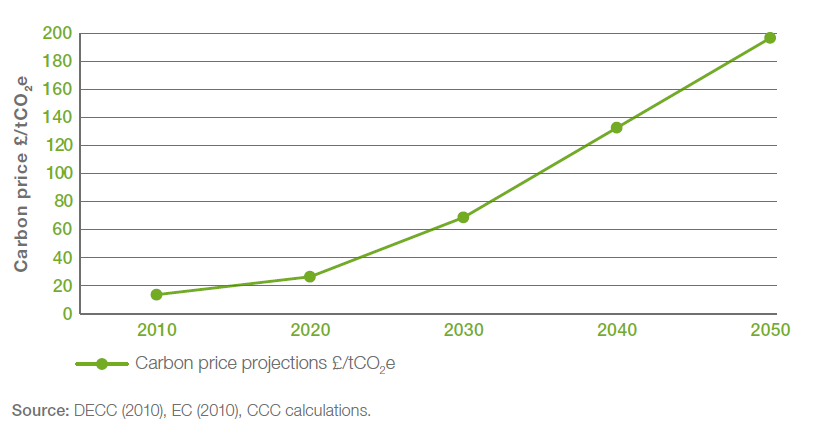
\includegraphics[height=6cm]{projection.png}
\end{center}
}


\frame{
\frametitle{Employing the instruments we learned}
\begin{itemize}
\item Carbon pricing is a tax: A trade-off between market efficiency and clean environment?
\item Is carbon pricing a Pareto improvement or not?
\item Is carbon pricing fair?
\item More importantly: Can it be effective?
\end{itemize}
}



\frame{
\frametitle{Problems}
\begin{itemize}
\item Problem of collective action. E.U. Emissions Trading Scheme is already below 30GBP
\item What impact on developing countries?
\item Who should get these tax revenues?

\end{itemize}
}

\frame{
\frametitle{Conclusion}
\begin{center}
There's no such thing as a simple solution
\end{center}
}

\end{document}
